\documentclass[conference]{IEEEtran}

\usepackage{amsmath}
\usepackage{booktabs}
\usepackage{cite}
\usepackage{graphicx}
\usepackage{hyperref}
\usepackage{microtype}
\usepackage{pgfplots}
\usepackage{tikz}
\usepackage{xcolor}
\pgfplotsset{compat=1.18}
\usetikzlibrary{arrows.meta,fit,positioning}

\title{Work-Aware Bucketed NUTS:\\
When Chain Scheduling Reduces Straggler Time}
\author{\IEEEauthorblockN{Viktor Najdovski}
\IEEEauthorblockA{Faculty of Computer Science and Engineering\\
Ss.\ Cyril and Methodius University\\
Skopje, North Macedonia\\
viktornajdovski@students.finki.ukim.mk}}

\begin{document}
\maketitle

\begin{abstract}
The No-U-Turn Sampler (NUTS) constructs a trajectory whose length depends on
local geometry.  In a vectorized multi-chain implementation, one unusually deep
trajectory can therefore keep an entire batch active after the other chains
have stopped.  We study a scheduling layer that predicts each chain's tree
depth, sorts chains by expected work, and executes fixed-shape buckets with
independent termination conditions.  The scheduler does not alter the
per-chain transition or its random-number stream.

The central result is a mechanism-and-limits result, not a general accelerator
speedup.  After repairing data-dependent control flow and the U-turn criterion,
monolithic and bucketed execution agree on states, random keys, realized depth,
leapfrog count, acceptance, divergence, and maximum-depth status under shared
keys.  An acceptance-calibrated CPU suite uses five sampler seeds and 30 blocked
warm repetitions per configuration.  Of 36 bucketed configurations, 6 (16.7\%)
have median speedup above one; the median, best, and worst are $0.896\times$,
$1.059\times$, and $0.529\times$.  A controlled scaling study identifies an
amortization boundary: at 1024 chains, the best preconfigured funnel and
Gaussian-process rows reach $1.312\times$ and $1.136\times$, with hierarchical
bootstrap intervals wholly above one, while their 128-chain rows are slower.
Tail diagnostics show why average prediction error is incomplete: last-depth
prediction has lower error and better deepest-decile recall than an exponential
history predictor, but does not consistently improve scheduling.  A
non-deployable current-depth oracle retains $1.474\times$ focused headroom.
A100 MIG timings fail one-bucket controls and are rejected.  Work-aware
bucketing helps only when predictable straggler work is large enough to
amortize planning, movement, and narrower sequential execution.
\end{abstract}

\section{Introduction}

The No-U-Turn Sampler (NUTS) removes the need to choose a fixed Hamiltonian
trajectory length by doubling a binary trajectory until it turns back,
diverges, or reaches a depth limit \cite{hoffman2014nuts}.  This adaptivity is
statistically useful and computationally irregular.  When independent chains
are transformed into one vectorized program, the batch loop continues while
any chain remains active.  Finished lanes are masked, but the program retains
the width and trip count imposed by the slowest chain.  This synchronization
effect is a known obstacle for vectorized dynamic MCMC
\cite{radul2020autobatching,dance2025fsm}.

This paper asks whether a smaller intervention can recover part of that loss:
can chains with similar expected trajectory lengths be placed in separate
fixed-shape termination domains without changing NUTS itself?  The proposed
method predicts per-chain work from recent history, sorts the chains, pads them
to canonical bucket widths, and runs each bucket's vectorized NUTS loop until
that bucket---rather than the entire population---finishes.  We call the design \emph{work-aware bucketed NUTS}.  The evaluated
single-device executor scans buckets sequentially; ``bucketed'' therefore
refers to independent termination domains, not concurrent kernels.

The investigation produced a less flattering but more informative answer than
the original performance hypothesis.  Three implementation and measurement
controls materially changed the conclusion.  First, a trace-time-unrolled
transition executed the maximum tree regardless of realized depth, leaving no
straggler work for any scheduler to recover.  Second, a reversed backward-span
U-turn check made tree depth depend on a direction coin flip rather than target
geometry.  Third, step sizes selected to expose scheduling headroom produced
acceptance near one and made NUTS perform avoidable work.  Results before the
control-flow and U-turn repairs are excluded; results from under-tuned step
sizes are retained only as diagnostic evidence.

The contributions are consequently methodological as well as empirical:

\begin{itemize}
  \item a data-dependent JAX NUTS transition and a compiled, fixed-shape bucket
        executor in which each bucket has an independent stopping condition;
  \item deterministic equivalence tests that cover random keys, continuous and
        discrete transition metrics, Gaussian-process regression, and padded
        lane noninterference;
  \item a separation of transition work, scheduler quality, and wall-clock
        overhead using causal and non-causal planning controls; and
  \item a claim-bounded evaluation that reports positive, neutral, and negative
        rows, rejects failed GPU controls, and exposes the confounding effect of
        ordinary NUTS step-size adaptation.
\end{itemize}

The final finding is conditional.  Bucketing can reclaim real synchronization
work while preserving the Markov transition.  The available online predictor
and fixed scheduling costs, however, prevent that mechanism from becoming a
consistent end-to-end improvement in the measured regime.

\section{Background and Related Work}

NUTS recursively combines Hamiltonian subtrees and stops when its trajectory
begins to double back \cite{hoffman2014nuts}.  Iterative formulations make the
recursive construction compatible with staged computation
\cite{lao2020tfpmcmc}.  They do not by themselves remove the synchronization
cost of placing variable-length chains under one batched loop.

Program-counter autobatching attacks this broader class of divergent programs
by tracking the control-flow state of every batch member and advancing members
at compatible program points \cite{radul2020autobatching}.  More recently,
finite-state-machine transformations have been used to restructure dynamic MCMC
algorithms, including NUTS, for vectorized accelerators \cite{dance2025fsm}.
Those approaches transform the transition program.  Bucketed NUTS instead
retains one common per-chain transition and changes only which independent
chains share a batched termination condition.

This is more constrained than ordinary sorting of jobs by known runtime.
Trajectory work is unknown before execution, assignment changes at every MCMC
transition, and prediction errors affect cost through bucket maxima rather than
only average error.  Reordering must preserve each chain's transition and random
stream; padded lanes must not affect real state; and JAX compilation requires a
small set of fixed rectangular shapes.  These statistical, random-number, and
staging constraints define the scheduling problem addressed here.

A complementary direction replaces dynamic trajectories with algorithms whose
structure is more regular on accelerators.  ChEES-HMC adapts a fixed trajectory
length \cite{hoffman2021chees}; SNAPER-HMC adapts trajectory length around a
principal component \cite{sountsov2022snaper}; and MEADS uses a multi-chain
ensemble construction \cite{hoffman2022meads}.  These methods can be preferable
when throughput is the primary design constraint.  Our narrower question is
whether the original NUTS transition can be retained exactly while its
independent chains are scheduled more efficiently.

\section{Work Model}
\label{sec:work-model}

Let $C$ denote the number of chains and $L_{i,t}$ the realized leapfrog work of
chain $i$ at transition $t$.  A vectorized \texttt{while\_loop} continues while
any lane is active.  A useful proxy for monolithic executed lane-work is
\begin{equation}
  W_{\mathrm{mono},t}=C\max_{1\leq i\leq C}L_{i,t}.
  \label{eq:mono-work}
\end{equation}
For a fixed-shape partition $\mathcal{B}_t$, with physical width $S_b$ including
padding, independent bucket termination gives
\begin{equation}
  W_{\mathrm{bucket},t}=\sum_{b\in\mathcal{B}_t}
       S_b\max_{i\in b}L_{i,t},
  \qquad
  r_W=\frac{\sum_t W_{\mathrm{bucket},t}}
           {\sum_t W_{\mathrm{mono},t}}.
  \label{eq:bucket-work}
\end{equation}
The proxy is not a hardware instruction count: it treats every lane-step as
equal and can overstate work after some lanes within a subtree stop.  It is
nevertheless deterministic, hardware independent, and uses the same
approximation on both sides.  A ratio $r_W<1$ establishes the mechanism---the
schedule reduces the maximum-driven lane budget---but not a speedup.  Prediction,
sorting, gather, scatter, padding, narrower vector widths, and sequential bucket
execution all have to be paid from the saved work.

\section{Method}
\label{sec:method}

\subsection{Per-chain transition}

The implementation uses a fixed-step NUTS transition with identity mass matrix
in the reported experiments.  Each transition samples momentum, draws a slice
variable, doubles a trajectory in a randomly chosen direction, performs
leapfrog integration, and selects among slice-valid proposals by reservoir
sampling.  It stops on a U-turn, divergence, or maximum tree depth.  The
divergence threshold is 1000.

Trajectory doubling and subtree construction are expressed as JAX
\texttt{lax.while\_loop}s with data-dependent predicates.  A checkpoint stack
tests the classic recursive U-turn criterion on aligned power-of-two blocks.
The implementation intentionally does not add the generalized cross-subtree
criterion.  The direction of every span is normalized before its endpoint
momenta are tested; this is necessary because reversing the endpoint order
otherwise makes a backward step appear to turn immediately.

Early exit must not alter subsequent random numbers.  The earlier unrolled
reference split its trajectory key at every possible tree depth even after a
chain became inactive.  The control-flow transition therefore advances the
unused splits before returning.  It avoids discarded leapfrog work while
preserving the per-chain key sequence.

\subsection{Prediction and host planning}

The primary online predictor is an exponential moving average of previous
realized tree depths,
\begin{equation}
  \widehat d_{i,t}=\beta\widehat d_{i,t-1}
       +(1-\beta)d_{i,t-1}, \qquad \beta=0.9.
  \label{eq:history}
\end{equation}
The host performs a stable sort by $\widehat d_{i,t}$ and packs the result into
canonical widths.  It chooses capacities by minimum padding and then minimum
bucket count.  Equal scores yield the original chain order; this is the
``none'' or unsorted control.

Two additional planners isolate scheduler quality.  \emph{Oracle-previous}
sorts by the immediately preceding realized depth.  It is causal, but is used
as a diagnostic rather than the primary policy.  \emph{Oracle-current} sorts by
the depth about to be realized in the current transition.  That information is
unavailable online, so oracle-current is an analysis-only upper bound and is
never counted as deployable evidence.

The plan is a rectangular index array plus a validity mask.  Padding repeats a
real source index so that an invalid lane cannot become the deepest member of a
bucket.  During scatter, invalid lanes are routed to an out-of-bounds row and
dropped.  They cannot overwrite a real state, metric, or random key.

\subsection{Fixed-shape executor}

Monolithic execution applies the per-chain transition with \texttt{vmap} over
all $C$ chains.  Bucketed execution gathers the rectangle and applies
\texttt{lax.map} over its bucket axis; each mapped element contains a
\texttt{vmap} over that bucket's lanes.  This distinction is essential.
Flattening the rectangle, or vectorizing the bucket axis, would place all
buckets under one global \texttt{any(active)} predicate and restore the
monolithic maximum.

The production path compiles gather, bucket map, and masked scatter as one JIT
program.  The instrumented benchmark path uses separately compiled gather,
executor, and scatter calls so their times can be observed.  It still has no
Python loop or accelerator dispatch per bucket: the sequential bucket scan is
inside the compiled \texttt{lax.map}.  It does, however, pay the structural cost
of executing several narrower loops rather than one wide loop.

Figure~\ref{fig:architecture} summarizes the evaluated architecture.

\begin{figure*}[t]
  \centering
  \resizebox{0.94\textwidth}{!}{%
  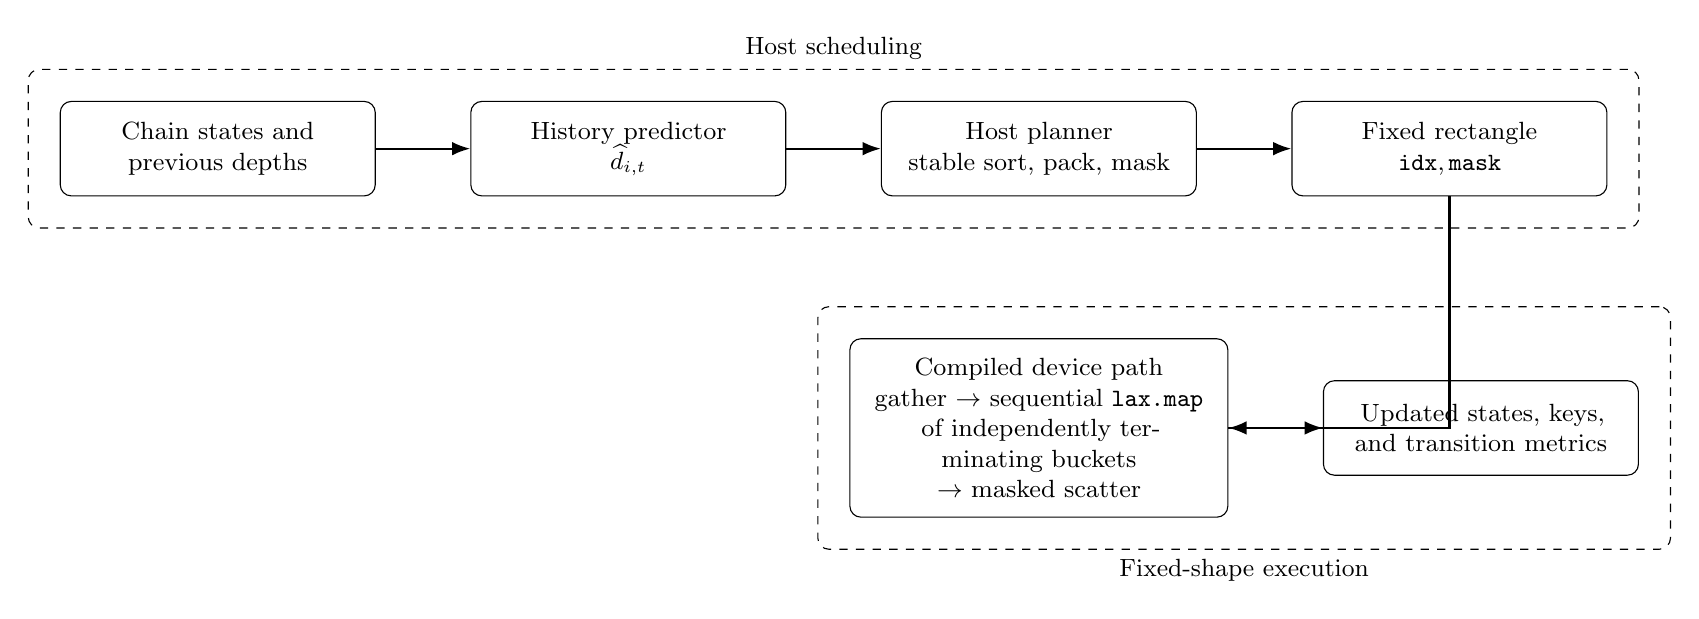
\begin{tikzpicture}[
    font=\small,
    box/.style={draw,rounded corners,align=center,minimum height=12mm,
                text width=35mm,inner sep=2.5mm},
    arr/.style={-Latex,thick},
    node distance=12mm
  ]
    \node[box] (state) {Chain states and\\previous depths};
    \node[box,right=of state] (predict) {History predictor\\$\widehat d_{i,t}$};
    \node[box,right=of predict] (plan) {Host planner\\stable sort, pack, mask};
    \node[box,right=of plan] (rect) {Fixed rectangle\\$\mathtt{idx},\mathtt{mask}$};
    \node[box,below=18mm of plan,text width=43mm] (exec)
      {Compiled device path\\gather $\rightarrow$ sequential \texttt{lax.map}\\
       of independently terminating buckets\\$\rightarrow$ masked scatter};
    \node[box,right=of exec] (next) {Updated states, keys,\\and transition metrics};
    \draw[arr] (state)--(predict);
    \draw[arr] (predict)--(plan);
    \draw[arr] (plan)--(rect);
    \draw[arr] (rect.south) |- (exec.east);
    \draw[arr] (exec)--(next);
    \node[draw,dashed,rounded corners,fit=(state)(predict)(plan)(rect),
          inner sep=4mm,label=above:{Host scheduling}] {};
    \node[draw,dashed,rounded corners,fit=(exec)(next),
          inner sep=4mm,label=below:{Fixed-shape execution}] {};
  \end{tikzpicture}}
  \caption{Work-aware bucketed NUTS.  Planning is host-side.  The compiled
  executor gives each bucket a separate batched termination condition.  In the
  evaluated single-device implementation the bucket map is sequential, not
  concurrent.}
  \label{fig:architecture}
\end{figure*}

\section{Evidence Discipline and Experimental Design}
\label{sec:design}

\subsection{Evidence audit}

The repository contains several generations of outputs.  Treating all of them
as exchangeable would produce a strong but false result.  Table~\ref{tab:ledger}
records the inclusion rule used in this paper.

\begin{table*}[t]
\centering
\caption{Evidence ledger.  Excluded artifacts remain available for diagnosis
but do not support final performance claims.}
\label{tab:ledger}
\small
\begin{tabular}{p{0.19\textwidth}p{0.25\textwidth}p{0.47\textwidth}}
\toprule
Evidence generation & Status & Reason and permitted use \\
\midrule
Run 21070 and other pre-repair sweeps & Excluded & The transition was fully
unrolled, so realized depth did not control executed work; later audits also
found a shared U-turn defect.  Run 21070 is negative diagnostic evidence only:
21/735 bucketed rows were faster, median speedup was $0.244\times$, and 35/45
Gaussian-process rows had leapfrog-count mismatches. \\
Pre-T43 mechanism experiments & Excluded & They established useful engineering
tests but used a U-turn rule that made backward subtrees stop incorrectly.  All
performance magnitudes and posterior diagnostics from this generation are void. \\
Post-repair, step size 0.03 funnel runs & Diagnostic & The transition is valid,
but mean acceptance is 0.997 on the focused CPU target.  These runs quantify the
adaptation confound and are not headline evidence. \\
Initial T51 timing pass & Excluded & The first untimed production call was
inside the retained sample, so one of 30 observations contained compilation.
The raw pass is preserved under \path{results/raw/t51_preferred/}; no value from
it is used in the revised headline. \\
T51-v2 acceptance-calibrated CPU suite and scaling study & Included & These are
post-repair, float32 measurements with an explicit cold priming call followed by
five sampler seeds and 30 fully blocked warm repetitions per configuration.
Step sizes were selected independently from bucketing performance.  The earlier
focused CPU oracle gap remains a secondary mechanism decomposition. \\
A100 MIG runs 23078--23079 & Rejected & One-bucket controls with identical
executed work differ by up to $1.78\times$ in time.  No GPU wall-clock number is
used as evidence. \\
\bottomrule
\end{tabular}
\end{table*}

This ledger also resolves the earlier draft target of approximately
$1.28\times$ at $C=2048$, $D=128$ on an A100.  The current codebase does not
reproduce that result under a valid protocol, and this paper makes no such
claim.

\subsection{Correctness protocol}

Monolithic and bucketed paths start from identical positions and identical
per-chain random keys.  Tests compare positions, final keys, realized tree
depth, leapfrog count, divergence and maximum-depth flags, acceptance
statistic, energy error, and gradient norm.  Keys and discrete metrics must be
exact.  Floating-point fields use absolute and relative tolerances of
$10^{-5}$; the tolerance covers compiler reordering in differential tests and
is not weakened per model.  A poisoned-padding test verifies that invalid lanes
cannot affect any real output.

Agreement between two wrappers cannot validate their shared transition.  The
suite therefore also compares the control-flow implementation with a preserved
unrolled reference, compares the checkpoint U-turn rule with an independent
brute-force recursion over aligned subtrees, checks forward/backward symmetry,
and tests that realized depth responds to target scale.  A minimal exact
Gaussian-process regression case guards the mismatch family discovered in run
21070.

\subsection{Timing protocol}

Every JAX result is passed through a tree-wide \texttt{block\_until\_ready}
before the wall clock is read.  Cold execution is separated from warm
execution.  Each T51 configuration retains all 30 blocked warm measurements of
the complete 16-transition workload and reports their median and interquartile
range.  Five sampler seeds vary initial positions and transition random streams
while model data remain fixed.  Methods are timed sequentially, so equal repeat
indices are not treated as paired observations.

For each configuration, speedup is first computed from the monolithic and
bucketed timing medians within each seed, then summarized by the median across
seeds.  A deterministic 10,000-draw hierarchical bootstrap resamples seeds and
the two methods' retained timing samples independently; reported 95\% intervals
are percentile intervals.  They are configuration-level descriptive intervals
and are not corrected for selecting the best row.  Speedup is always
\begin{equation}
  \mathrm{speedup}=t_{\mathrm{mono}}/t_{\mathrm{bucket}}.
\end{equation}

\subsection{Final CPU suite}

Experiments ran on eight virtual CPU cores backed by an Intel Xeon E7-8880 v3
at 2.30 GHz, under Linux, Python 3.10.12, JAX 0.4.38, and jaxlib 0.4.38.  All
reported arrays are float32.  Each model uses five sampler seeds, $C=512$
chains, 16 transitions, maximum tree depth 8, and bucket widths 64 and 128.  Six
bucketed configurations are evaluated per model: unsorted, exponential-history,
and last-realized-depth planning at each width.  Last-depth is causal: only work
from the chain's preceding transition is used.

Step sizes were selected in a separate coarse CPU calibration by proximity to
the conventional 0.8 dual-averaging acceptance target, not by bucketed
speedup.  Table~\ref{tab:models} reports the calibrated values and final
transition diagnostics.  Several calibration points lie at the edge of the
swept range, and the centered Eight Schools and Gaussian-process workloads have
non-negligible divergence counts.  The experiment is consequently a scheduling
microbenchmark, not evidence of posterior accuracy.

\begin{table*}[t]
\centering
\caption{Acceptance-calibrated CPU workloads.  Warm time and divergences are
medians over five sampler seeds; divergence ranges appear in brackets.  Each
seed contains $512\times16=8192$ transitions, and discrete metrics match every
bucketed configuration.}
\label{tab:models}
\small
\resizebox{0.98\textwidth}{!}{%
\begin{tabular}{lrrrrrr}
\toprule
Target & Dimension & Step size & Calibration accept. & Monolithic warm (s) & Divergences & Max depth \\
\midrule
Funnel & 4 & 0.20 & 0.867 & 1.068 & 8 [4,14] & 8 \\
Eight Schools, centered & 10 & 0.30 & 0.728 & 1.767 & 431 [423,439] & 8 \\
Eight Schools, noncentered & 10 & 0.60 & 0.798 & 0.410 & 11 [8,15] & 5 \\
Gaussian process ($N=8$) & 3 & 0.20 & 0.727 & 3.961 & 62 [52,76] & 6 \\
Stochastic volatility & 6 & 0.20 & 0.725 & 0.316 & 0 [0,0] & 5 \\
Hierarchical logistic & 8 & 0.50 & 0.767 & 0.381 & 1 [0,2] & 5 \\
\bottomrule
\end{tabular}
}
\end{table*}

A focused mechanism experiment uses the funnel with $C=512$, $D=32$, 16
transitions, step size 0.2, depth limit 8, and the same two bucket widths.  It adds the causal last-depth policy (called \texttt{oracle\_previous} in the
raw schema for historical reasons) and an analysis-only current-depth oracle.
Its calibration acceptance is 0.867.  Its wall-clock decomposition predates T51
and uses one seed and minimum-of-three timing, so it is secondary mechanism
evidence rather than the statistical headline.

\section{Results}
\label{sec:results}

\subsection{Transition preservation}

The current regression suite passes all monolithic--bucketed equivalence,
control-flow differential, U-turn ground-truth, and padding tests.  In the
Gaussian-process gate, final keys and every discrete transition metric are
exact, while continuous values satisfy the fixed $10^{-5}$ tolerance.  More
importantly for the final performance data, all 180 bucketed seed/configuration
rows (six models, five seeds, six configurations) have exactly the same
aggregate leapfrog count as their corresponding monolithic run.  The mismatch
count is zero for every model family.

The scheduler therefore changes execution organization, not the per-chain
transition under the tested configuration.  Identical transitions imply
identical effective samples per iteration for matched streams, but the short
timing suite does not estimate ESS or convergence independently.

\subsection{Six-model wall-clock results}

Table~\ref{tab:suite-results} reports the fastest of six preconfigured
bucketed configurations per model.  This best-row view is descriptive; the
aggregate over all configurations is the primary guard against selection.
Across the 36 model/policy/width configurations, 6 have median speedup above one
(16.7\%).  The best, median, and worst are $1.059\times$, $0.896\times$, and
$0.529\times$.  The best row exceeds one for three of six model families, but
only funnel has a best-row interval whose lower endpoint is above one.  Across
all rows, three individual configuration intervals lie wholly above one: funnel
history/64 and centered Eight Schools history/128 and last-depth/128.  No
multiplicity correction is applied.

\begin{table*}[t]
\centering
\caption{Fastest preconfigured bucketed configuration per model.  Values are
medians across five seeds; intervals hierarchically resample seeds and 30 warm
timings per method.  Best-row selection is descriptive.}
\label{tab:suite-results}
\small
\begin{tabular}{lrrrr}
\toprule
Model & Median speedup & 95\% CI & Predictor & Width \\
\midrule
eight\_schools\_centered & 1.038 & [0.970, 1.116] & unsorted & 128 \\
eight\_schools\_noncentered & 0.955 & [0.894, 1.148] & unsorted & 128 \\
funnel & 1.059 & [1.008, 1.149] & history & 64 \\
gaussian\_process & 1.019 & [0.934, 1.119] & unsorted & 128 \\
hierarchical\_logistic & 0.884 & [0.769, 1.090] & unsorted & 64 \\
stochastic\_volatility & 0.686 & [0.448, 0.887] & last-depth & 128 \\
\bottomrule
\end{tabular}

\end{table*}

The stronger timing protocol materially narrows the earlier one-seed result.
Funnel history at width 64 is now $1.059\times$ with interval
$[1.008,1.149]$, while the best Gaussian-process row is $1.019\times$ with
interval $[0.934,1.119]$.  Centered Eight Schools at width 128 reaches
$1.030\times$ $[1.019,1.106]$ for history and $1.036\times$
$[1.017,1.116]$ for causal last-depth.  Most configurations remain slower, so the data do not support
a general CPU acceleration claim.

\subsection{Controlled chain-count scaling}

A post-repair scaling study holds each target, step size, transition count, and
policy set fixed while varying $C\in\{128,256,512,1024\}$.  Table
\ref{tab:scaling} reports the best of four preconfigured history/last-depth and
width-64/128 rows at each chain count.  The selection caveat is the same as for
Table~\ref{tab:suite-results}.

\begin{table*}[t]
\centering
\caption{Controlled CPU chain scaling with five seeds and 30 warm repetitions.
Intervals are hierarchical 95\% bootstrap intervals.}
\label{tab:scaling}
\small
\begin{tabular}{lrrrr}
\toprule
Model & Chains & Median speedup & 95\% CI & Policy/width \\
\midrule
funnel & 128 & 0.963 & [0.760, 1.064] & last-depth/64 \\
funnel & 256 & 0.904 & [0.819, 0.964] & history/128 \\
funnel & 512 & 1.006 & [0.841, 1.054] & history/128 \\
funnel & 1024 & 1.312 & [1.227, 1.434] & history/128 \\
gaussian\_process & 128 & 0.929 & [0.859, 1.009] & last-depth/128 \\
gaussian\_process & 256 & 0.960 & [0.892, 0.992] & history/64 \\
gaussian\_process & 512 & 1.008 & [0.981, 1.129] & last-depth/128 \\
gaussian\_process & 1024 & 1.136 & [1.027, 1.173] & last-depth/64 \\
\bottomrule
\end{tabular}

\end{table*}

The amortization boundary is visible on both targets.  At $C=128$, the best
funnel and Gaussian-process rows are slower at $0.963\times$ and
$0.929\times$.  At $C=1024$, they reach $1.312\times$
$[1.227,1.434]$ and $1.136\times$ $[1.027,1.173]$, respectively.
Gaussian-process speedup rises steadily across the four chain counts; funnel is
noisier at intermediate counts but changes decisively at 1024.  This controlled
result supports the systems interpretation more directly than correlation
across unrelated targets: fixed scheduling costs become easier to amortize as
the chain population and reclaimable straggler budget grow.

\subsection{Predictor ordering and the straggler tail}

The focused funnel calibration output records every predicted and realized
depth for five seeds.  Table~\ref{tab:predictor-diagnostics} reports per-step
Spearman correlation, recall of the deepest 10\% of chains, realized-depth range
within predicted buckets, and mean absolute error.  Tail sets use a stable
rank-based top decile; depth ties are therefore resolved deterministically.

\begin{table*}[t]
\centering
\caption{Five-seed predictor diagnostics on the acceptance-calibrated focused
funnel.  Oracle-current is non-deployable.  Bucket range is the mean realized
maximum-minus-minimum depth after sorting by predicted work.}
\label{tab:predictor-diagnostics}
\small
\begin{tabular}{lrrrrr}
\toprule
Predictor & Width & Spearman & Tail recall & Bucket range & MAE \\
\midrule
history & 64 & 0.594 & 0.492 & 1.783 & 1.288 \\
history & 128 & 0.594 & 0.492 & 2.031 & 1.288 \\
last-depth & 64 & 0.631 & 0.672 & 1.905 & 0.307 \\
last-depth & 128 & 0.631 & 0.672 & 2.147 & 0.307 \\
oracle-current & 64 & 1.000 & 1.000 & 0.408 & 0.000 \\
oracle-current & 128 & 1.000 & 1.000 & 0.816 & 0.000 \\
\bottomrule
\end{tabular}

\end{table*}

Last-depth improves mean absolute error from 1.288 to 0.307, per-step Spearman
correlation from 0.594 to 0.631, and deepest-decile recall from 0.492 to 0.672.
Yet its mean within-bucket depth range is slightly worse than history at both
widths, and the six-model suite does not show a consistent last-depth advantage.
Depth itself has lag-one correlation 0.756.  These results sharpen the
predictor finding: causal signal exists, but global rank accuracy and low MAE do
not guarantee compact maxima in every fixed-width bucket.  Scheduler objectives
should target the straggler tail and resulting bucket maxima directly.

\subsection{Mechanism and oracle gap}

The focused funnel separates reduced work from reduced time.  Table
\ref{tab:oracle-gap} shows that every planner reduces the lane-work proxy, but
not every row is faster.  The primary history scheduler at width 64 executes
0.528 of monolithic lane-work and reaches $1.042\times$.  This falls below the
pre-specified $1.05\times$ primary gate.  At width 128 it is slower.  The causal
last-depth diagnostic is also unstable across widths: it reaches
$1.073\times$ at width 128 but $0.957\times$ at width 64.

\begin{table}[t]
\centering
\caption{Focused acceptance-calibrated funnel ($C=512$, $D=32$).  Monolithic
warm time is 0.661 s.  Oracle-current uses future information and is
analysis-only.}
\label{tab:oracle-gap}
\small
\begin{tabular}{lrrr}
\toprule
Planner & Width & Work ratio $r_W$ & Speedup \\
\midrule
History & 64 & 0.528 & 1.042 \\
History & 128 & 0.593 & 0.974 \\
Last-depth & 64 & 0.543 & 0.957 \\
Last-depth & 128 & 0.599 & 1.073 \\
Oracle-current & 64 & 0.347 & \textbf{1.474} \\
Oracle-current & 128 & 0.441 & 1.215 \\
\bottomrule
\end{tabular}
\end{table}

\begin{figure}[t]
\centering
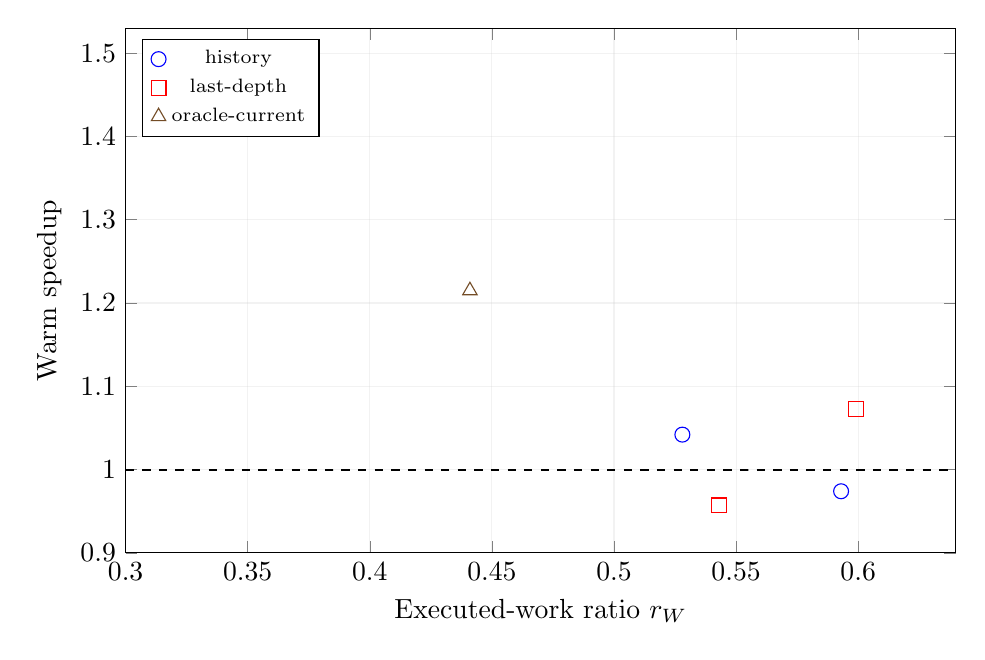
\begin{tikzpicture}
\begin{axis}[
  width=\columnwidth,
  height=0.68\columnwidth,
  xmin=0.30,xmax=0.64,
  ymin=0.90,ymax=1.53,
  xlabel={Executed-work ratio $r_W$},
  ylabel={Warm speedup},
  grid=both,
  grid style={opacity=0.2},
  legend style={font=\scriptsize,at={(0.02,0.98)},anchor=north west}
]
\addplot+[only marks,mark=o,mark size=2.7pt] coordinates {
  (0.528,1.042) (0.593,0.974)
};
\addlegendentry{history}
\addplot+[only marks,mark=square,mark size=2.7pt] coordinates {
  (0.543,0.957) (0.599,1.073)
};
\addlegendentry{last-depth}
\addplot+[only marks,mark=triangle,mark size=3pt] coordinates {
  (0.347,1.474) (0.441,1.215)
};
\addlegendentry{oracle-current}
\addplot[black,dashed,thick,domain=0.30:0.64] {1};
\end{axis}
\end{tikzpicture}
\caption{Lower lane-work is useful but not sufficient for lower wall time.
Oracle-current is a non-deployable upper bound.}
\label{fig:oracle-gap}
\end{figure}

The current-depth oracle demonstrates that the executor can turn a sufficiently
good partition into end-to-end speedup: $r_W=0.347$ becomes $1.474\times$ even
after planning and movement.  History leaves a substantial prediction gap,
with mean absolute depth error about 1.29 and $r_W=0.528$ for the same width.
The five-seed diagnostics above show that last-depth has much lower average
error yet still produces a similar focused work ratio.  The bucket-max objective
is more demanding than average depth prediction.

Diagnostic component timers reinforce, but do not precisely add up to, this
account.  For history at width 64 they record 64 ms planning, 3 ms gather,
17 ms scatter, and 527 ms executor time over the 16-transition workload.  The
authoritative outer warm total is 634 ms against 661 ms monolithic.  The saved
executor budget is therefore thin enough that host planning and data movement
can erase it.  These pre-T51 component fields are retained only for qualitative
attribution; they are not combined with the new timing intervals.

\subsection{Adaptation is a competing optimization}

The same focused funnel exposes a central confound.  With step size 0.03, mean
acceptance is 0.997 and monolithic warm time is approximately 1.31 s.  In that
regime, history rows produced roughly $1.19\times$--$1.29\times$ and the
analysis-only oracle reached still larger values.  At step size 0.2, mean
acceptance is 0.867, monolithic time falls to 0.661 s, and the primary history
speedup falls to $1.042\times$.

Thus bucketing can appear to recover work that ordinary dual-averaging would
avoid by increasing the step size.  Choosing a step size to maximize
reclaimable work tunes the benchmark toward the scheduler.  The final evidence
uses acceptance as an independent selection criterion and treats the larger
under-tuned speedups only as a sensitivity result.  Predictor engineering and
sampler adaptation should be evaluated jointly, not as separable sources of
speedup.

\subsection{GPU timings fail their controls}
\label{sec:gpu}

The acceptance-calibrated A100 MIG run at $C=2048$, $D=128$ contains an
apparently favorable history row: two buckets of width 1024 report
$1.301\times$.  It cannot be accepted.  A one-bucket row has no partitioning
mechanism and should behave like monolithic execution plus modest wrapper cost.
Instead, one-bucket history and one-bucket oracle-current execute exactly the
same 974,848 lane-steps but take 2.303 s and 1.292 s, respectively, a
$1.78\times$ spread.  Across one-bucket controls, nominal speedups range from
$0.802\times$ to $1.429\times$.  Moreover, moving from the adjacent under-tuned
run to the acceptance-calibrated run reduces the work proxy by $3.93\times$ but
increases monolithic time from 1.446 s to 1.846 s.

The assigned MIG instance was dedicated to the benchmark, so the inconsistency
cannot simply be assigned to another process on the same device.  Scheduler-
specific compilation or layout, the minimum-repeat protocol, and instrumentation
organization remain possible causes, but the available data do not distinguish
them.  Under the pre-established one-bucket control, every GPU wall-clock row is
rejected.  There is no valid GPU speedup or slowdown result in this paper.

\section{Discussion}

\subsection{What is established}

The corrected program demonstrates the proposed mechanism.  Once trajectory
work is genuinely data dependent, grouping similar chains into separate
termination domains reduces a deterministic lane-work proxy.  Shared-key tests
show that this reorganization preserves the transition, including its random
stream and padding behavior.  An oracle partition converts the reduction into
as much as $1.474\times$ end-to-end CPU speedup on the focused, acceptance-
calibrated target.

The deployable result is narrower.  Only 6 of 36 final configurations have
median speedup above one, the median row is an 11.5\% slowdown, and most
configuration-level intervals include or lie below one.  The controlled scaling
study nevertheless shows a reproducible positive regime at 1024 chains.
Prediction must compact the deepest chains within fixed buckets, not merely
obtain low average error.  Even then, fixed host planning and movement must fit
inside the difference between monolithic and bucket executor time.

\subsection{The single-device execution trade-off}

Independent bucket exit requires independent loop regions.  Fusing all lanes
under one \texttt{vmap} restores a single shared predicate and therefore the
global straggler.  The current \texttt{lax.map} preserves independent exit by
scanning buckets, which reduces SIMD width and can sacrifice occupancy.  This
trade-off is mild enough for some CPU workloads and potentially severe on a
GPU.  Concurrent bucket programs or multi-device sharding are possible future
designs, but they require a fair multi-device monolithic baseline and new
controls.  They are not results of the present implementation.

\subsection{Lessons from the failed generations}

The pre-repair history illustrates three general systems lessons.  First,
semantic equivalence between two wrappers cannot detect a defect in their
shared transition; independent ground-truth tests are necessary.  Second, a
scheduler benchmark must prove that realized work changes executed work before
interpreting wall time.  Third, an optimization should be evaluated after the
baseline's own adaptation has removed avoidable work.  Without these controls,
the same project appeared to support both large speedups and large slowdowns,
neither of which described the final method.

\section{Limitations}

The final evaluation uses five seeds and 30 repetitions, but it remains a short
systems microbenchmark: 16-transition windows, six small model instances, and
two scaling targets.  Step sizes are coarsely calibrated, not produced by an
integrated dual-averaging warmup; the mass matrix is not adapted.  The centered
Eight Schools and Gaussian-process configurations retain divergences, so the
suite should not be used for posterior-quality comparisons.  No long-chain ESS,
$\widehat R$, or effective samples per gradient evaluation are reported.
Bootstrap intervals quantify timing and seed variation under this protocol, not
model or hardware generalization, and best-row intervals are not adjusted for
selection.

The executed-work ratio in Eq.~\eqref{eq:bucket-work} is a model of batched
lane-steps rather than a device counter.  The T51 headline uses the production
outer path without component synchronization; older component measurements are
diagnostic and need not add exactly to the new totals.  The results therefore
support qualitative mechanism attribution but not a precise cycle-level cost
model.

The checkpoint implementation follows the classic recursive U-turn blocks and
does not implement a generalized cross-subtree criterion.  Its level checks can
be expensive when the target gradient itself is cheap, although that cost is
shared by the compared paths.  Finally, the evaluated executor is sequential
across buckets and all valid performance evidence is CPU-only.  Accelerator
performance, scaling beyond 1024 chains and two targets, and concurrent bucket
execution remain unresolved.

\section{Reproducibility}

The preferred suite is stored under
\path{results/raw/t51_preferred_v2/final_suite/}; scaling outputs are under
\path{results/raw/t51_preferred_v2/scaling/}; and five-seed predictor calibration
is under \path{results/raw/t51_preferred/predictor_diagnostics/}.  Every
headline configuration includes \path{timing_repetitions.csv}; processed CSV,
JSON, and LaTeX tables are generated under
\path{results/processed/t51_preferred_v2/}.  The focused decomposition remains
under \path{results/raw/oracle_gap/accept_targeted_cpu/}, and the repaired
Gaussian-process gate is under
\path{results/raw/correctness/gp_tiny_uturn_fixed/}.  Manifests record resolved
profiles, configuration hashes, Python and platform metadata, row counts, and
the 30-repeat median timing rule.  Rejected GPU artifacts are preserved under
run IDs 23078 and 23079 rather than overwritten; concurrently generated GPU
work is not used by this revision.

\section{Conclusion}

Work-aware bucketed NUTS is a valid work-reclamation mechanism, but the
evidence does not support a broad acceleration claim.  The repaired scheduler
preserves the tested NUTS transition and can substantially reduce maximum-driven
lane-work.  Under five seeds and 30 blocked repetitions, only 6 of 36 final
configurations have median speedup above one; the median is $0.896\times$ and
the best is $1.059\times$.  The controlled scaling study identifies the useful
regime more clearly: best preconfigured rows at 1024 chains reach
$1.312\times$ on the funnel and $1.136\times$ on the Gaussian process, with
intervals above one, after being slower at 128 chains.  A non-deployable
current-depth oracle retains $1.474\times$ focused headroom.  The gap is the
result: predictable heterogeneity and sufficient scale create headroom, but
prediction error, host planning, data movement, and narrower sequential
execution consume most of it.  Proper step-size calibration further
shrinks the opportunity by removing work that a tuned NUTS baseline would not
perform.  GPU timings fail internal controls and remain an open question.

The defensible conclusion is therefore conditional and falsifiable: bucketed
scheduling can help when per-chain work is persistent enough to predict and
expensive enough to amortize scheduling, but it is counterproductive outside
that regime.  Establishing the mechanism, its correctness, and its limits is
the final contribution of this study.

\begin{thebibliography}{99}

\bibitem{hoffman2014nuts}
M.~D. Hoffman and A.~Gelman, ``The No-U-Turn Sampler: Adaptively Setting Path
Lengths in Hamiltonian Monte Carlo,'' \emph{Journal of Machine Learning
Research}, vol.~15, no.~47, pp.~1593--1623, 2014.

\bibitem{radul2020autobatching}
A.~Radul, B.~Patton, D.~Maclaurin, M.~D. Hoffman, and R.~A. Saurous,
``Automatically Batching Control-Intensive Programs for Modern Accelerators,''
in \emph{Proc. Machine Learning and Systems (MLSys)}, 2020.

\bibitem{lao2020tfpmcmc}
J.~Lao, C.~Suter, I.~Langmore, C.~Chimisov, A.~Saxena, P.~Sountsov, D.~Moore,
R.~A. Saurous, M.~D. Hoffman, and J.~V. Dillon, ``tfp.mcmc: Modern Markov Chain
Monte Carlo Tools Built for Modern Hardware,'' \emph{arXiv:2002.01184}, 2020.

\bibitem{dance2025fsm}
H.~Dance, P.~Glaser, P.~Orbanz, and R.~P. Adams, ``Efficiently Vectorized MCMC
on Modern Accelerators,'' in \emph{Proc. 42nd International Conference on
Machine Learning}, PMLR, vol.~267, pp.~12436--12458, 2025.

\bibitem{hoffman2021chees}
M.~D. Hoffman, P.~Sountsov, J.~V. Dillon, and R.~A. Saurous, ``An Adaptive-MCMC
Scheme for Setting Trajectory Lengths in Hamiltonian Monte Carlo,'' in
\emph{Proc. AISTATS}, 2021.

\bibitem{sountsov2022snaper}
P.~Sountsov and M.~D. Hoffman, ``SNAPER-HMC: Adaptive Step Size and Path Length
for Efficient Hamiltonian Monte Carlo,'' \emph{arXiv:2205.12588}, 2022.

\bibitem{hoffman2022meads}
M.~D. Hoffman and P.~Sountsov, ``MEADS: Multi-Chain Ensemble Adaptive Dynamic
Sampling,'' \emph{arXiv:2210.10936}, 2022.

\end{thebibliography}

\end{document}
